\chapter{Feasibility study}

As already mentioned, the main motivation behind the thesis is derived from the observation that the existing methods of vessel destination prediction neglect data depth in their models. Especially, not considering the type and dimensions of vessels is presumed to be a major limitation of the existing literature. In order to establish this in an empirical manner, a feasibility study was conducted on the aspect of \acrfull{mo}'s novel segmentation of vessels. As part of the course work for the prior \acrshort{ntnu} course called \textit{“IMT4894 Advanced Project Work”}, such a feasibility study was  conducted to estimate the impact of vessel segmentation on the aspect of port frequencies. Port frequencies, or patterns of port arrivals and departures should reflect the fact that different vessels of different types travel in different patterns. Thus, if it is possible to show that segmentations have a significant impact on these patterns through port frequencies, it can be concluded that it will have an impact on vessel destination predictions.

The dataset used in this feasibility study mainly consisted of vessel transitions (as described in \cref{sec:vessel_transitions}), and port data (as described in \cref{sec:port_data}). The dataset also includes the vessel's segment and sub-segment (as described in \cref{sec:vessel_segments}). For a given port, every visiting vessel was assigned the attribute \textit{NextPort} that indicated the next arrival port after departing the given port. \cref{fig:apw_dataset} shows an example of vessels arriving at the port of Oslo (\texttt{NOOSL}).

\begin{figure}[htbp]
    \centering
    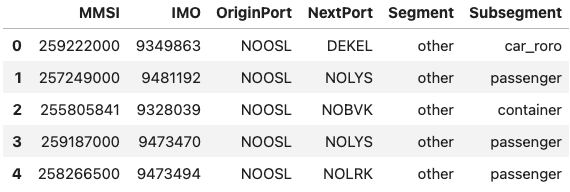
\includegraphics[width=.8\textwidth]{figures/apw/apw_dataset.png}
    \caption{A sample of the dataset used in the feasibility study}
    \label{fig:apw_dataset}
\end{figure}

In the feasibility study, there were two main steps in the analysis process. Firstly, a single-case analysis was conducted on a port known to the author to establish a more thorough overview of the traveling patterns of different vessel types and to gain an understanding of how to interpret the results. Secondly, a trend analysis was conducted on a collection of ports in order to establish a recurring pattern. In the study, a few major ports were selected combined with a few ports known to the author and experts in \acrshort{mo}. The complete list of ports are listed in \cref{sec:trend_analysis}.

\section{Single-case analysis}

For the single-case analysis, the port of Oslo (\texttt{NOOSL}) was selected as it is frequented by both dry bulk cargo vessels as well as several passenger vessels. It was presumed that the higher traveling frequency of the passenger vessels would heavily skew the most frequent next port for all vessels visiting \texttt{NOOSL}. Firstly, the distribution of the next frequented ports from the port was mapped as shown in \cref{fig:apw_noosl_freq} which shows that the port of Lysaker (\texttt{NOLYS}) is the most frequented next port by far. Lysaker port is a very small port that mostly receives passenger vessels that, as expected, would have high frequency because passenger vessels frequently travel back and forth over short distances. This also means that few passenger vessels could be responsible for almost all voyages, and predictions would be heavily skewed toward \texttt{NOLYS}.

\begin{figure}[htbp]
    \centering
    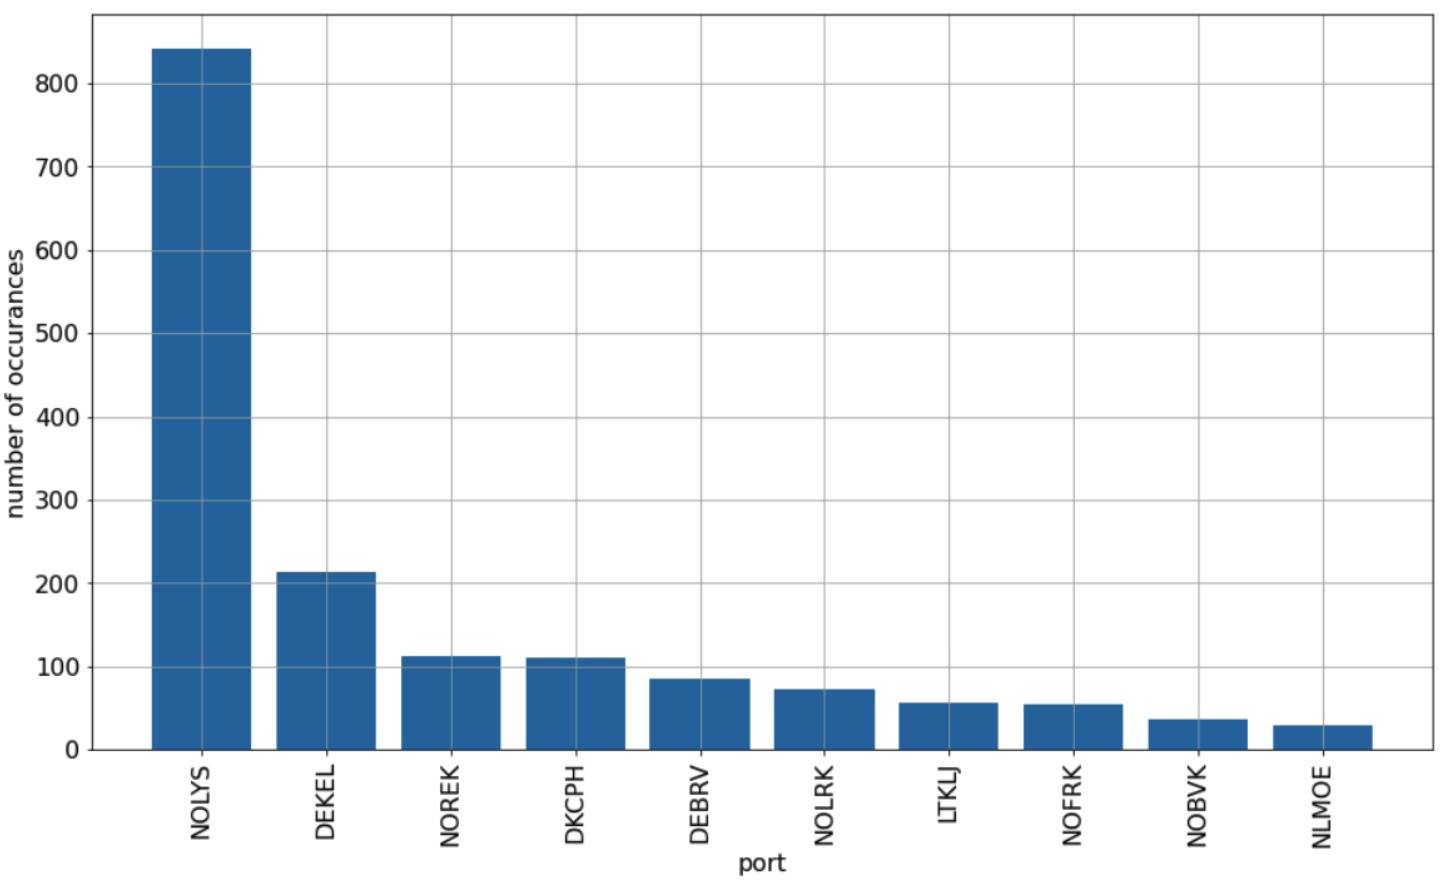
\includegraphics[width=.9\textwidth]{figures/apw/noosl_freq.png}
    \caption{Distribution of \textit{NextPort}s from \texttt{NOOSL}}
    \label{fig:apw_noosl_freq}
\end{figure}

When looking into the distributions of \textit{NextPort}s per segment it is even more apparent that the \textit{Other} segment (which includes passenger vessels) are responsible for the high number of voyages to \texttt{NOLYS}. \cref{fig:apw_noosl_segments} shows this as well as the \textit{Other} is the only segment that shares the same most frequent next port \texttt{NOLYS}. This means that a prediction algorithm using port frequencies would accurately predict the next destination ports for these other vessels, but not for the rest. Since the other vessels are responsible for 1568 out of 2009 transitions (78.05\%), considering vessel segmentation for predictions, and assuming every vessel always travel to its segment most frequent next port, a prediction algorithm could also become accurate for the remainder of the vessel segments which adds up to 21.95\% of all transition and probably most of the unique vessels. This is the basis used to estimate an improvement, or impact, factor for vessel segmentation on destination predictions.

\begin{figure}[htbp]
    \centering
    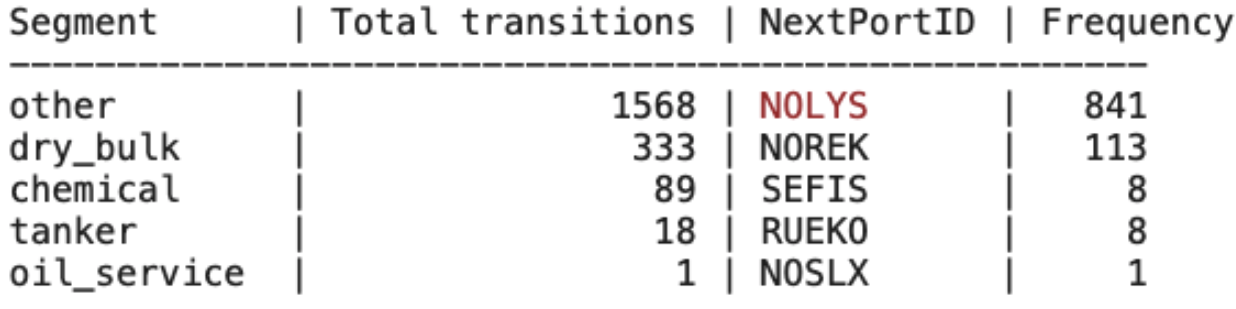
\includegraphics[width=.7\textwidth]{figures/apw/noosl_segments.png}
    \caption{Distribution of \textit{NextPort}s from \texttt{NOOSL} per segment}
    \label{fig:apw_noosl_segments}
\end{figure}

Furthermore, as \cref{fig:apw_noosl_dry_bulk} shows, when looking at the port frequency of the dry bulk cargo vessels, it is apparent that \texttt{NOLYS} is not even a contender for the most frequent next port. Therefore, a prediction method considering port frequencies would not be able to accurately predict the next destination port for any other vessel other than passenger vessels.

\begin{figure}[htbp]
    \centering
    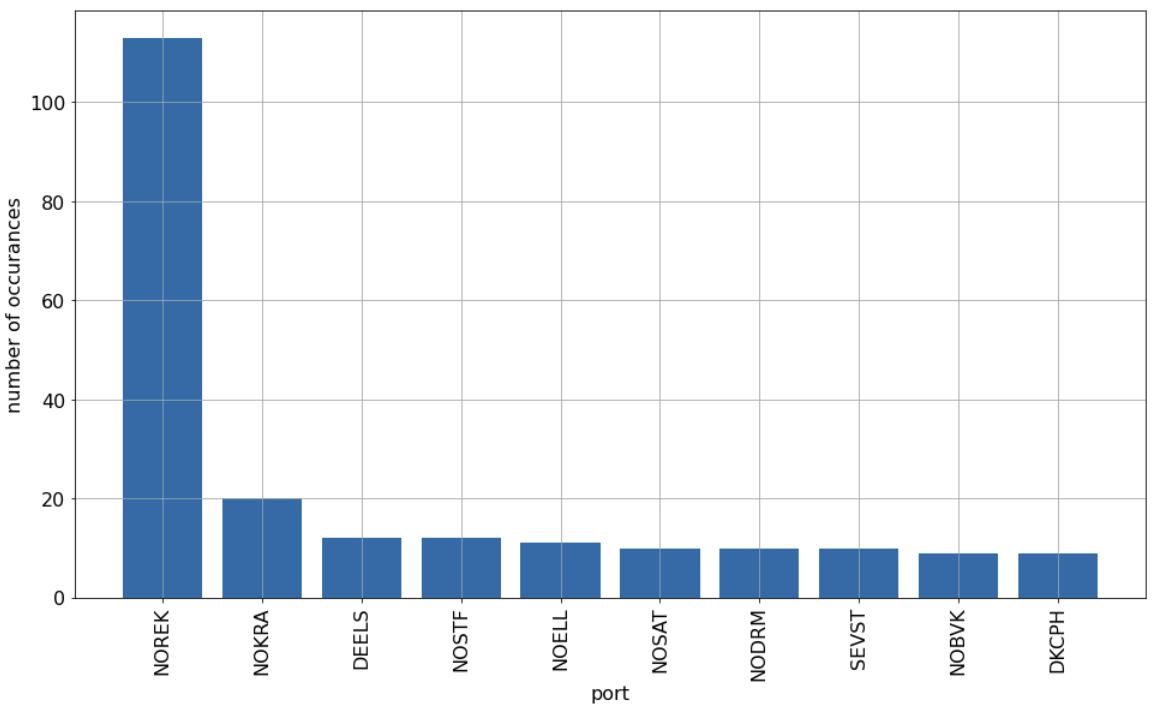
\includegraphics[width=.9\textwidth]{figures/apw/noosl_dry_bulk.png}
    \caption{Distribution of \textit{NextPort}s from \texttt{NOOSL} for the \textit{`dry bulk' segment}\label{fig:apw_noosl_dry_bulk}}
\end{figure}

Investigating sub-segments further confirms that a few numbers of vessels are responsible for most of all total transitions. \cref{fig:apw_noosl_subsegments} shows that the specific sub-segment \textit{`other - passenger'}, or passenger vessels, are responsible for 49.52\% of all transitions and nearly all voyages arrive at \texttt{NOLYS} after \texttt{NOOSL}. This means a prediction model could potentially be improved by 50\% if it would be aware of the sub-segment of each vessel for this particular port. \texttt{NOOSL} seems to be a port that shows the problem area quite well because it is a smaller port that receives a lower number of different vessels, and when there are multiple passenger vessels frequently arriving at it, they heavily skew the results in their favor.% chktex 8

\begin{figure}[htbp]
    \centering
    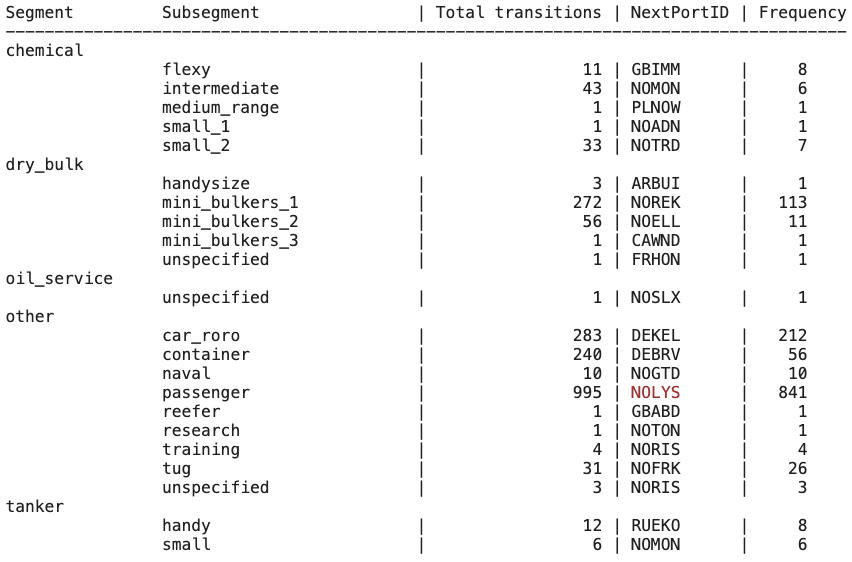
\includegraphics[width=.8\textwidth]{figures/apw/noosl_subsegments.png}
    \caption{Distribution of \textit{NextPort}s from \texttt{NOOSL} per sub-segment}
    \label{fig:apw_noosl_subsegments}
\end{figure}


\section{Trend analysis}
\label{sec:trend_analysis}

As already mentioned, for the trend analysis, a number of ports were selected based on their size and traffic. There were also a couple of known ports included in this dataset to easier interpret the results. The ports used in the analysis were:

\begin{itemize}
    \item \texttt{NLRTM} --- Rotterdam, Netherlands
    \item \texttt{NOOSL} --- Oslo, Norway
    \item \texttt{CNSHG} --- Shanghai, China
    \item \texttt{NLMSV} --- Maasvlakte, Netherlands
    \item \texttt{SGSIN} --- Singapore, Singapore
    \item \texttt{USHPY} --- Baytown, USA
    \item \texttt{BEANR} --- Antwerpen, Belgium
    \item \texttt{TWKHH} --- Kaohsiung, Taiwan
    \item \texttt{JPYOK} --- Yokohama
\end{itemize}

The same process as for the single-case analysis was conducted, but on a higher level as the main purpose of this study was to establish a trend in terms of a impact factor of vessel segmentation on port frequencies. \cref{fig:trend_freq} shows a similar version of the table used for the single port analysis (\cref{fig:apw_noosl_freq}) but also shows the number of transitions that differed from the most frequent next port when considering segments (i.e.\ the estimated improvement factor).

\begin{figure}[htbp]
    \centering
    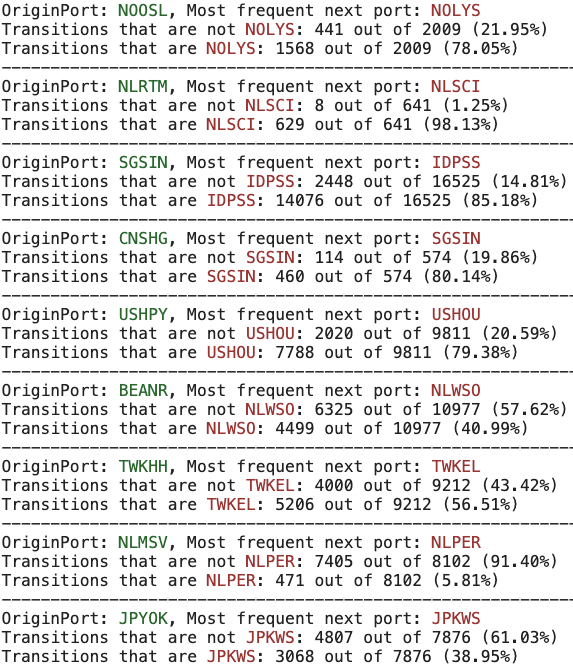
\includegraphics[width=.56\textwidth]{figures/apw/trend_frequency.png}
    \caption{Port frequencies and transition distribution as they relate to the most frequent next port for the selected ports}
    \label{fig:trend_freq}
\end{figure}

\begin{figure}[htbp]
    \centering
    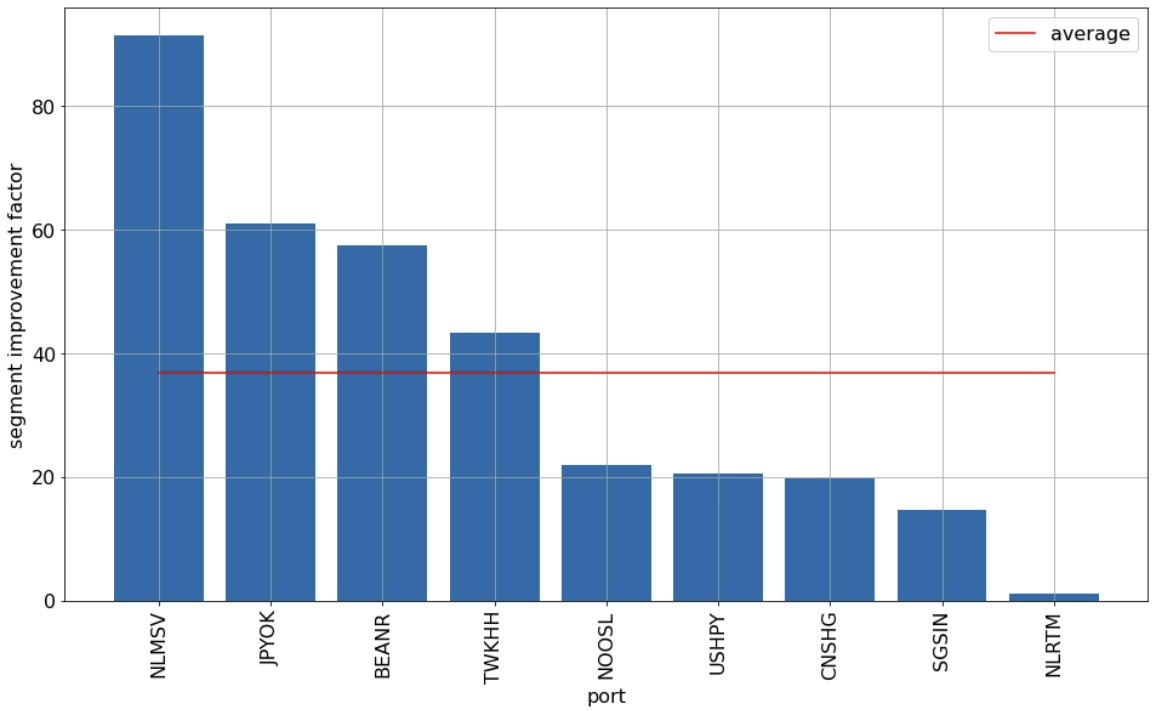
\includegraphics[width=.9\textwidth]{figures/apw/segment_improvement.png}
    \caption{Distribution of improvement factors for each origin port considering segments}
    \label{fig:segment_improvment}
\end{figure}

It is apparent that there are variances in improvement factors for different ports ranging from as low as \textit{1.25\%} to as high as \textit{91.40\%}. In the case of \texttt{NLRTM}, which is mostly a dry bulk port, there were no considerable improvements as almost all vessels are of the same segment. For the port \texttt{NLMSV}, the opposite was the case as there were a plethora of different types of vessels that frequented the port. \cref{fig:segment_improvment} shows the distribution of the improvement factor considering segments for each origin port as well as the overall average impact factor for these 9 ports which was \textit{36.88\%}.

Furthermore, when looking at the impact of sub-segments, as \cref{fig:subsegment_improvment} shows, it seems that the improvement factor has increased overall. For example, in the case of \texttt{NLRTM}, the improvement factor has increased from \textit{1.25\%} to \textit{19.66\%}, and although this varied for the different ports, the overall average improvement factor increased from \textit{36.88\%} to \textit{50.28\%}.

\begin{figure}[htbp]
    \centering
    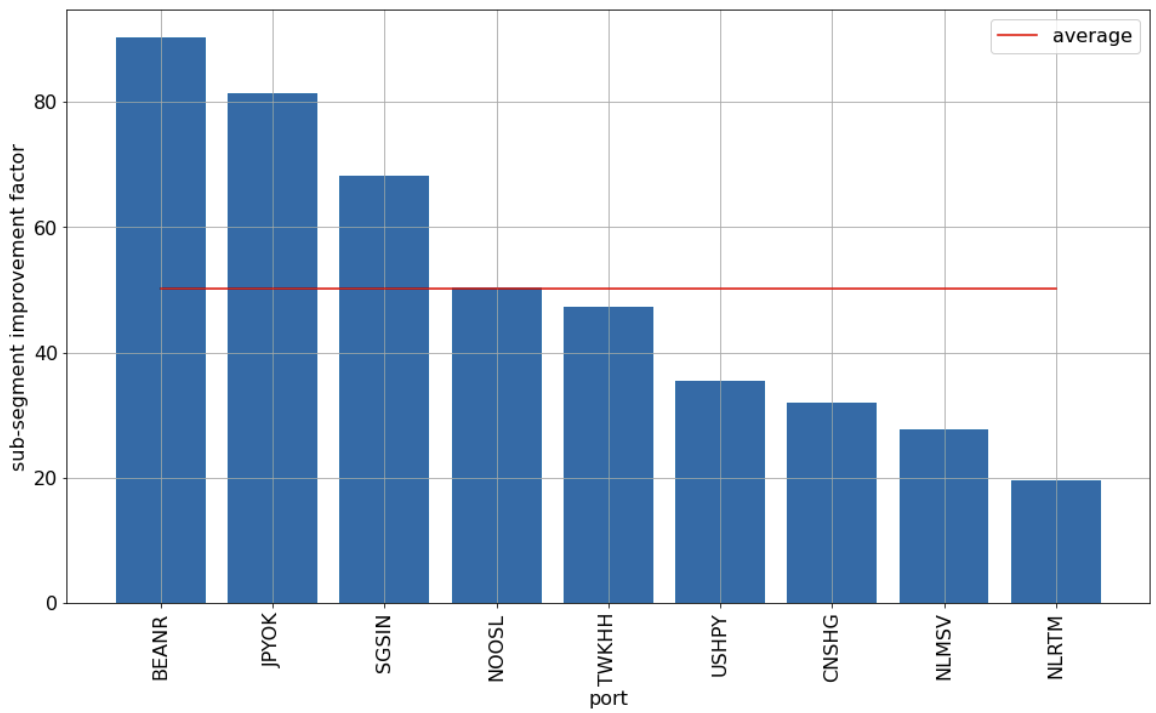
\includegraphics[width=.9\textwidth]{figures/apw/subsegment_improvement.png}
    \caption{Distribution of improvement factors for each origin port considering sub-segments}
    \label{fig:subsegment_improvment}
\end{figure}

A prediction method considering the frequencies of ports for vessel destination predictions would choose the most frequent next port for the predicted next destination. In this scenario, ignoring the vessel's type (segmentation) would give the wrong prediction for a lot of vessels from different segments in a lot of ports. The results from the feasibility study clearly indicates that applying the aspect of vessel segmentation to such models would definitively have an impact on prediction accuracy and, therefore, is worth investigating further. Moreover, assuming this impact would also, to some degree, apply to vessel trajectories as they relate to traveling patters, improving the accuracy of a model such as the one described in~\cite{ZHANG2020102729} seems to be plausible depending on the data foundation.
